\section{Vizualizace myšlenkových map}
\label{vizualizcemap}
O zobrazování myšlenkových map se stará knihovna V-network-graph. Práce s ní byla vcelku přímočará, veškeré informace jsem čerpal z oficiální dokumentace s ukázkami \cite{vnetexamples}. Postupně jsem si z jednotlivých ukázek zaměřených vždy na jednu problematiku vybral, co potřebuji, a sestavil jsem z toho finální komplexní nástroj.
\newline
Samotná knihovna poskytuje následující funkce:
\begin{enumerate}
    \item zoom
    \item přesouvání se po mapě
    \item přidávání a odebírání vrcholu
    \item přidávání a odebírán hrany
    \item podpora customizace - barvy, velikosti, animace vrhcolů a hran
    \item dynamické překreslování (například při změně barvy vrcholu)
    \item interagování s grafem
    \item integrace force layoutu pomocí D3.js
    \item zobrazení mřížky
\end{enumerate}
\newpage
Jak již bylo zmíněno, vše dohromady přichází k "životu" v souboru \textit{MapNetwork.vue} . Veškerá funkcionalita a interaktivita s grafem je zřízena v souboru \textit{graphManager.js}, nacházející se zde funkce pro správu vrcholů, hran atd. Ukázka \ref{nodeadd} dává za příklad jednoduchou funkci pro přidání nového vrcholu. Vypočítá nové id a namapuje hodnoty pro nový vrchol. 
\begin{lstlisting}[style=JavaScript, firstnumber = 5, caption={utils/graphManager.js, přidání vrcholu do grafu},
label={nodeadd}]
// adds a new node to the graph
function addNewNode(data, nodeProps, xMousePos, yMousePos) {
    // Find the largest numeric part of the existing keys
    const maxNodeId = findCurrentMaxNodeId(data);
    // Generate the next key
    const nextNodeId = `node${maxNodeId + 1}`;
    
    // Add the new node with all properties
    data.nodes[nextNodeId] = {
        name: nodeProps.name,
        color: nodeProps.color,
        size: nodeProps.size
    };
    // Adds the new node to the layouts so its position is tracked
    data.layouts.nodes[nextNodeId] = { x: xMousePos, y: yMousePos };
    
    historyManager.addToHistory(data);
    
}
\end{lstlisting}
Nachází se zde ale i komplikovanější funkce, například \textit{waveNodeSelect} viz ukázka \ref{wave}. Tato funkce rekurzivně přidává vrcholy, které jsou potomky těch již označených, do označených vrcholů. Tato funkcionalita rozšiřuje možnosti editace myšlenkových map.
\newpage
\begin{lstlisting}[style=JavaScript, firstnumber = 264, caption={utils/graphManager.js, wave select},
label={wave}]
// Function which will recusively select all the nodes connected to the selected node
async function waveNodeSelect(data, selectedNodes, callback) {
    const visited = new Set(selectedNodes);
    const newlySelected = [];
    
    // Get connected nodes that haven't been visited
    Object.values(data.edges).forEach(edge => {
        const source = edge.source;
        const target = edge.target;
        
        if (selectedNodes.includes(source) && !visited.has(target)) {
            visited.add(target);
            newlySelected.push(target);
        }
        if (selectedNodes.includes(target) && !visited.has(source)) {
            visited.add(source);
            newlySelected.push(source);
        }
    });

    if (newlySelected.length > 0) {
        callback(newlySelected);
    }
    
    return newlySelected;
}
\end{lstlisting}
Další zajímavá implementovaná funkce zařizuje automatické generování šířek a barev hran na základě spojených vrcholů. Tato funkce vždy vychází z většího vrcholu, přepočítá se jeho velikost na šířku hrany pomocí konstanty, dále hrana zdědí i barvu většího vrcholu; akorát má slabší alpha kanál, o tom se více dočtete v kapitole \ref{config}. Na ukázce \ref{edgeadd} je možno vidět tuto funkcionalitu ve funkci pro přidání hran mezi všemi vybranými vrcholy \textit{addEdges}.
\newpage
\begin{lstlisting}[style=JavaScript, firstnumber = 92, caption={utils/graphManager.js, přidání hran a jejich automatická konfigurace},
label={edgeadd}]
// Function which will add edges between all selected nodes
function addEdges(data, selectedNodes) {
    // Return if selected nodes are less than 2 - cannot create an edge
    if (selectedNodes.length < 2) return;
    
    const maxEdgeId = findCurrentMaxEdgeId(data);
    // Tracks how many new edges are created
    // So the next edge id can be generated
    let newEdgeCounter = 0;
    
    for (let srcIndex = 0; srcIndex < selectedNodes.length - 1; srcIndex++) {
        for (let trgtIndex = srcIndex + 1; trgtIndex < selectedNodes.length; trgtIndex++) {

            const source = selectedNodes[srcIndex];
            const target = selectedNodes[trgtIndex];
            if (!edgeExists(data, source, target)) {
                // Increase the counter by 1
                newEdgeCounter++;
                // Creates a new edge id
                const nextEdgeId = `edge${maxEdgeId + newEdgeCounter}`;
                const edgeProps = getLargerNodeProperties(data, source, target);
                data.edges[nextEdgeId] = { 
                    source, 
                    target, 
                    color: edgeProps.color,
                    width: edgeProps.width
                };
                // .....
\end{lstlisting}

\subsection{Implementace grafů}
Grafy jsem implementoval tak, v jaké podobě je vyžaduje V-network-graph, tedy v podobě 3 seznamů: \textit{nodes, edges, layouts}. Výsledný nástroj není koncipovaný pro velké množství záznamů v jednom grafu, nebylo tedy potřeba vytvářet žádnou speciální implementaci grafu. Ukázkový graf viz ukázka \ref{showcasedata}.
\newpage
\begin{lstlisting}[style=JavaScript, firstnumber = 1, caption={ Implemetnace ukázkového grafu},
label={showcasedata}]
const nodes: Nodes = {
  node1: { name: "Idea-Atlas", color: "#2c3e50", size: 100 },
  node2: { name: "Nuxt",color: "#2ecc71", size: 50  },
  node3: { name: "Vue", color: "#2ecc71", size: 30  },
  node4: { name: "Java Script", color: "#f1c40f", size: 30  }
}
const edges: Edges = {
  edge1: { source: "node1", target: "node2", color: "#2c3e50", width: 8 },
  edge2: { source: "node2", target: "node3", color: "#2ecc71", width: 4 },
  edge3: { source: "node4", target: "node2", color: "#2ecc71", width: 4 }
}
const layouts: Layouts = {
  nodes: {
    node1: { x: 200, y: 40 },
    node2: { x: -110, y: 80 },
    node3: { x: -410, y: 160 },
    node4: { x: -310, y: -160 }
  },
}
\end{lstlisting}
O trochu složitější graf pak může vypadat jako ten na obrázku \ref{fig:graph}.
\begin{figure}[h]
    \centering
    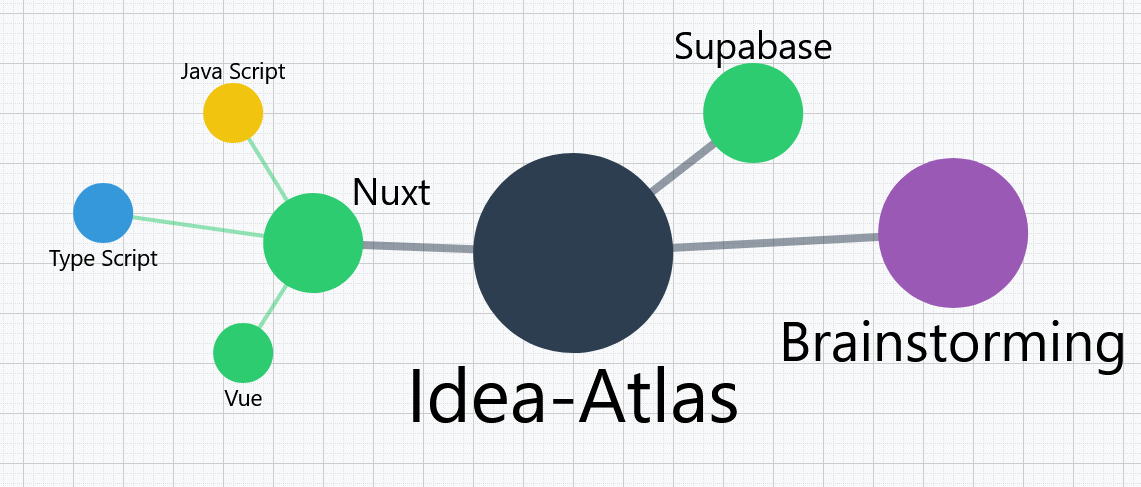
\includegraphics[width=1\linewidth]{Images/graph.png}
    \caption{Ukázkový graf}
    \label{fig:graph}
\end{figure}
\subsection{Konfigurace V-network-graph}
\label{config}
Konfigurace této knihovny hraje v mém projektu zásadní roli. Konfigurace se postupně měnila a rostla spolu s komplexitou projektu. Zejména se jedná o upravené, personalizované výtažky z dokumentace V-network-graph \cite{vnetexamples}. Kompletní konfigurační soubor \textit{mapNetworkConfig.ts} je k nalezení v adresáři \textit{config}.
\par
Na ukázce \ref{config1} se nachází první část konfigurace V-network-graph, konfiguruje se zde na příklad:
\begin{enumerate}
    \item zdali je povolen box selection a jak vypadá
    \item vzhled mřížky na pozadí
    \item vypnutí zvětšování objektů podle přiblížení
    \item minimální a maximální přiblížení, které může uživatel provést
    \item zakázání přiblížení při dvojitém kliku; v mém projektu má dvojtý klik funkci přidání nového uzlu
\end{enumerate}
\begin{lstlisting}[style=JavaScript, firstnumber = 56, caption={config/mapNetworkConfig.ts, první část konfigurace vNG},
label = {config1}]
view: {
    /...
      boxSelectionEnabled: true,
      selection: {
        box: {
          color: "#0000ff20",
          strokeWidth: 1,
          strokeColor: "#aaaaff",
          strokeDasharray: "0",
        },
      },
      grid: {
        visible: true,
        interval: 10,
        thickIncrements: 5,
        line: {
        //...
        },
        thick: {
          color: "#cccccc",
          width: 1,
          dasharray: 0,
        },
      },
      layoutHandler: new vNG.GridLayout({ grid: 10 }),
      scalingObjects: true,
      minZoomLevel: 0.1,
      maxZoomLevel: 16,
      doubleClickZoomEnabled: false,
    },
    /...
\end{lstlisting}
Na ukázce \ref{config2} se konfigurují vlastnosti a vzhled vrcholů:
\begin{enumerate}
    \item jak vypadá vrchol v normálním stavu
    \item jak se změní vrchol, když na něj uživatel najede myší
    \item jak vypadá popisek vrcholu; dále se tam zapíná automatické posouvání popisku, aby nepřekážel hranám, které vedou z daného vrcholu
\end{enumerate}
\begin{lstlisting}[style=JavaScript, firstnumber = 87, caption={config/mapNetworkConfig.ts, druhá část konfigurace vNG},
label = {config2}]
    node: {
      normal: {
        type: "circle",
        radius: node => node.size, // Use the value of each node object
        color: node => node.color,
      },
      hover: {
        radius: node => node.size + 4,
        color: node => node.color,
      },
      selectable: true,
      label: {
        visible: true,
        fontFamily: undefined,
        fontSize: node => calculateFontSize(node.size),
        lineHeight: 1.1,
        color: "#000000",
        margin: 4,
        direction: "south",
        directionAutoAdjustment: true,
        background: {
          visible: false,
          color: "#ffffff",
          padding: {
            vertical: 1,
            horizontal: 4,
          },
          borderRadius: 2,
        },
      },
    },
\end{lstlisting}
\newpage
Na ukázce \ref{config3} se nastavuje:
\begin{enumerate}
    \item zda se dají vybrat hrany
    \item jak vypadají hrany v normálním stavu
    \item co se stane s hranami, když na ně uživatel namíří myšítkem
    \item jak budou hrany vypadat, když je uživatel označí
\end{enumerate}
\begin{lstlisting}[style=JavaScript, firstnumber = 118, caption={config/mapNetworkConfig.ts, třetí část konfigurace vNG},
label = {config3}]
edge: {
      selectable: true,
      normal: {
        width: edge => edge.width, // Use the value of each edge object
        color: edge => convertToRGBA(edge.color),
      },
      hover: {
        width: edge => edge.width,
        color: edge => edge.color, // Use original color without transparency
      },
      selected: {
        width: edge => edge.width * 1.5, // Increase width by 50% when selected
        color: edge => edge.color,
        dasharray: "6",  // Fixed dash pattern for selected edges
        animate: true,   // Always animate selected edges
      },
    },
\end{lstlisting}

